

\subsection{Code-Quality-Benchmark mit anderen Ruby-Projekten}

Um die Ergebnisse besser einordnen zu können, vergleichen wir die Ergebnisse aus den Code-Quality-Benchmark mit vergangenen Ruby-Projekten in der pludoni GmbH und mit bekannten Ruby/Rails-OpenSource Software.

Eine vollständige Metrik wie oben, war in vielen Fällen nicht möglich, da die Testwerkzeuge in vielen Fällen Inkompatibilitäten mit neueren Rubyversionen haben. Wir beschränken uns deshalb auf eine exemplarische Überblicksmetrik, bestehend aus:

\begin{description}
 \item[LOC] Anzahl der Quellcodezeilen, gemessen durch das Rails-Kommando "`rake stats"'. 
 \item[LOT] Anzahl der Quellcodezeilen aller Tests, gemessen durch das Rails-Kommando "`rake stats"'. 
 \item[LOT/TOC] Verhältnis aus Testzeilen und Quellcodezeilen
 \item[AVGCmplx] Durchschnittliche Komplexität aller Klassen, gemessen durch \textbf{Flog}\footnote{\url{https://github.com/seattlerb/flog}}. Flog besitzt ein eigenes Maß für Code-Komplexität. Es vergibt für jede Zuweisungen, Verzweigungen und Funktionsaufrufe unterschiedlich viele Punkte, und bildet so eine Summe per Funktion oder per Klasse. Dabei vergibt Flog besonders viele Punkte für schwer nachzuvollziehende Funktionsaufrufe, wie z.B. "`eval(string)"', welches einen String als Ruby-Code auswertet.
 \item[H5Cmplx] Komplexität der 5\% komplexesten Klassen, nach Flog
 \item[DSmell] Anzahl der Code-Smells nach Roodi. Beinhaltet u.a.: hohe Cyclomatische Komplexität in einer Methode (min. 4), lange Methoden, lange Parameterlisten, u.v.m.\footnote{\url{http://roodi.rubyforge.org/files/README_txt.html}}
 \item[DSmell/KLOC] Anzahl der Code-Smells nach Roodi pro tausend Codezeilen
 \item[CSmell] Anzahl der Code-Smells nach Reek. Diese beinhalten: Geringe Kohäsion, Duplikation, Control-Couple, Unkommunikativer Name von Methoden/Variablen/Parameter, verschachtelte Iteratoren, u.v.m  \footnote{\url{https://github.com/kevinrutherford/reek/wiki/Code-Smells}}
 \item[CSmell/KLOC] Anzahl der Code-Smells nach Reek pro tausend Codezeilen
\end{description}
%Die Tools Roodi und Reek messen beide gewisse \glossarpl{smell}, die sich zum Teil überdecken.







\subsubsection{Vergleich von IT-Jobs-und-Stellen mit eigenen Projekten}

Bisherige Projekte der pludoni GmbH und des Autors basierend auf Ruby/ Ruby on Rails
\begin{description}
 \item[feedmerger] Eine Rails-Anwendung zur Verwalten, Cachen, Filtern und Zusammenfügen von RSS und Atom-Feeds. Als OpenSource unter \url{https://github.com/zealot128/WenShanWenHai} zu finden.
 \item[pludonidb] Ist eine auf ActiveRecord basierende Bibliothek zur Anbindung der Datenbanken der Communityportale an Ruby-Skripte. Beinhaltet außerdem weitere Hilfsfunktionen für diese Domäne.
 \item[backlinks] Backlink und SEO-Success-Control ist eine Rails-2.3 Anwendung, zum Messen der sogenannten Backlinks\footnote{TODO} der Communitymitglieder und der Platzierung für relevante Sucheingaben in den großen Suchmaschinen (konkret: Welchen Platz hatte ein Communityportal an einem bestimmten Tag für "`it jobs dresden"', usw.) %TODO Verweis auf meinen Praktikumsbericht
 \item[lpp] Linkpartnerprogramm ist eine Studenteninitiative der TU Dresden, um ausländische Studenten mit deutschen Sprach- und Lernpartnern zusammenzubringen. Dazu wurde 2008 von einem Studententeam im Rahmen einer Semesterarbeit eine Rails-Webanwendung geschrieben. Der Autor dieser Arbeit war zwar nicht an der Entwicklung beteiligt, übernahm aber die Pflege und Weiterentwicklung selbiger.
\end{description}


\begin{table}[hbp]
 \caption{Vergleich von IT-jobs mit anderen Ruby Projekten des Autors/der pludoni GmbH}\label{table:cmpmy}
 \begin{center}
 
\begin{tabular}{|l|l|l|l|l|l|l|}
\hline\rowcolor{tableheadcolor}

Projekt&ItJobs&Backlinks&Feedmerger&SAnalyzer&Feedimport&PludoniDb\\
\hline
Technologie&Rails3&Rails2&Rails3&Rails3&Ruby&Ruby\\
\hline
Testverfahren&TDD&manuell&manuell&manuell&TDD&manuell\\
\hline
LOC&1570&1884&724&214&571&1933\\
\hline
LOT&1750&75&137&0&865&126\\
\hline
LOT/LOC&1.11&0.04&0.19&0.00&1.51&0.07\\
\hline
AVGCmplx&8.00&19.90&10.50&14.80&16.80&13.70\\
\hline
H5Cmplx&43.80&70.60&26.90&39.70&25.10&113.20\\
\hline
DSemll&11&69&11&11&8&25\\
\hline
DSmell/KLOC&7.00&36.60&15.20&51.40&14.00&12.90\\
\hline
CSmell&53&152&52&13&28&113\\
\hline
CSmell/KLOC&33.80&80.70&71.80&60.70&49.00&58.50\\
\hline
\end{tabular}
\end{center}

\end{table}


\subsubsection{Vergleich von IT-Jobs-und-Stellen mit anderen Rails Projekten}
Weiterhin wird das Projekt mit folgenden beliebten Webprojekten, welche ebenfalls auf Ruby on Rails basieren, verglichen:
\begin{description}
 \item[diaspora] Ist ein verteiltes soziales Netzwerk. \\
 Code: \url{https://github.com/diaspora/diaspora}
 \item[bucketwise] ist ein web-basierter persönlicher Finanzmanager mit Budgetierung nach dem Briefumschlagsystem\\
 Code: \url{https://github.com/jamis/bucketwise}
 \item[chiliproject] Ist ein Fork\footnote{In der (Open-Source) Software-Entwicklung ist ein Fork eine legale Kopie eines bestehendes Software-Produktes, um von nun an eine unabhängige Entwicklung zu betreiben} des sehr beliebten Bugtrackers Redmine\footnote{https://github.com/edavis10/redmine}. Statt des originalen Redmines wurde dieser Fork genommen, da er eine neuere Codebasis hat\\
 Code: \url{https://github.com/chiliproject/chiliproject}
 \item[railscast] Ist der Code der Website \url{http://www.railscasts.com}, in welche allwöchentlich ein Screencast zum Thema Ruby und Rails veröffentlich wird (bis dato 283 Episoden).\\
 Code: \url{https://github.com/ryanb/railscasts} 
 \item[ActiveSupport] Beinhaltet Hilfsklassen und Erweiterungen der Standardbibliothek für \glossar{rails}. Kernbestandteil von Ruby on Rails \\
 Code: \url{https://github.com/rails/rails.git}
 \item[ActionPack]  ist Framework um Anfragen und Antworten eines Webservers zu verarbeiten und ist ein weiterer Kernbestandteil von Rails.\\
 Code: \url{https://github.com/rails/rails.git}
\end{description}

\begin{table}[hbp]
 \caption{Vergleich von IT-jobs mit Ruby/Rails Projekten aus der Community}\label{table:cmpother}
 \begin{tabular}{|p{1.8cm}|l|l|l|l|l|l|l|l|}
\hline \rowcolor{tableheadcolor}
 Projekt&itjobs&bucket&lpp&chili&aPack&aSupport&diaspora&rCasts\\
\hline
Technologie&Rails3&Rails2&Rails1&Rails2&Rails3&Rails3&Rails3&Rails3\\
\hline
LOC&1570&1979&7116&21201&12995&9407&7466&653\\
\hline
LOT&1750&1684&1557&20127&32570&13590&10072&748\\
\hline
LOT/LOC&1.11&0.85&0.22&0.95&2.51&1.44&1.35&1.15\\
\hline
AVGCmplx&8.00&12.80&17.10&19.10&11.10&10.90&13.10&11.00\\
\hline
H5Cmplx&43.80&32.20&181.80&84.40&64.00&47.90&54.00&34.60\\
\hline
DSmell&11&37&250&651&370&166&99&2\\
\hline
DSmell\newline~/KLOC&7.00&18.70&35.10&30.70&28.50&17.60&13.30&3.10\\
\hline
CSmell&53&129&386&1535&982&291&324&42\\
\hline
CSmell\newline~/KLOC&33.80&65.20&54.20&72.40&75.60&30.90&43.40&64.30\\
\hline
\end{tabular}
\end{table}

TODO Auswertung

\begin{figure}[htbp]
 \centering
 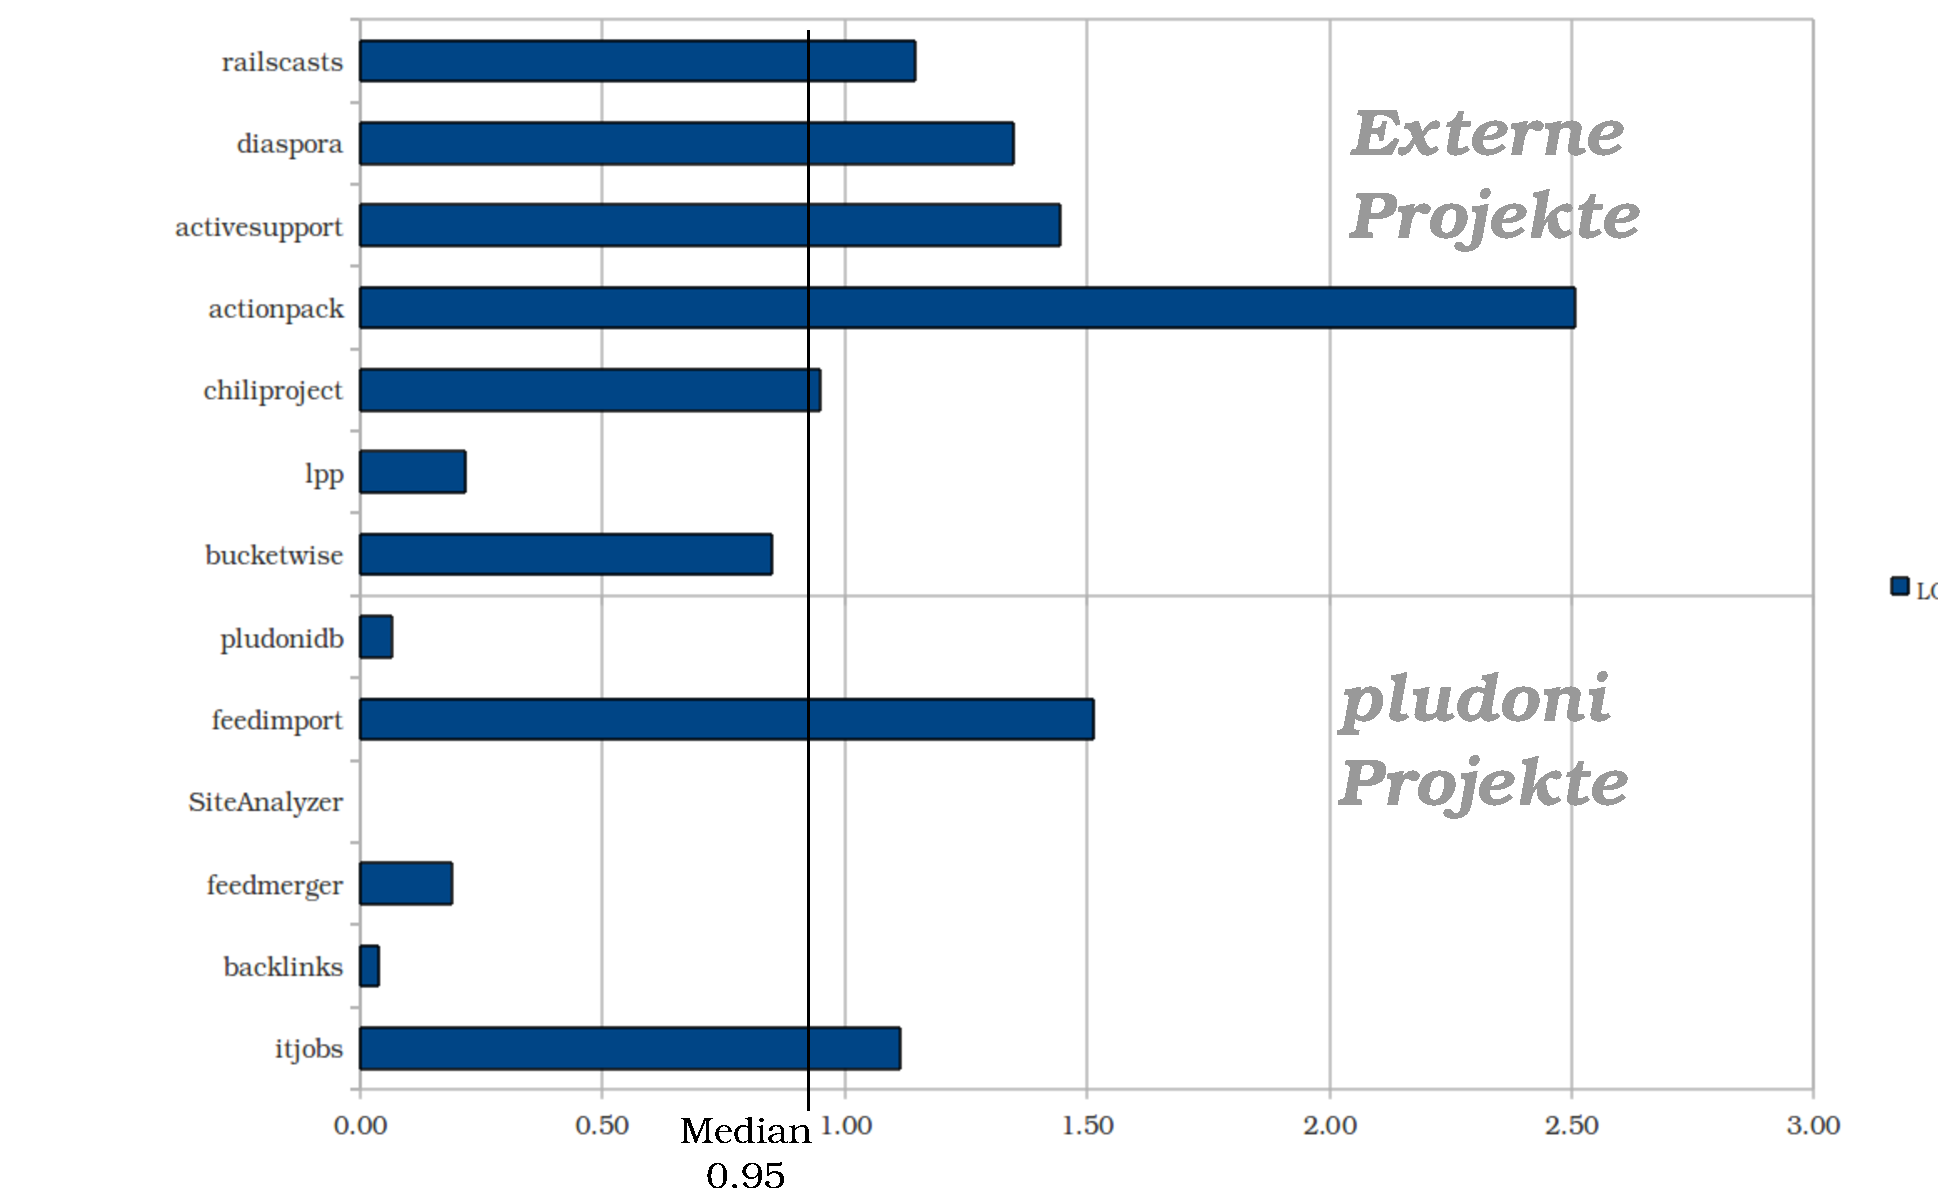
\includegraphics[width=\linewidth]{./diagrams/cpm-lotloc.pdf}
 % cpm-lotloc.pdf: 930x574 pixel, 72dpi, 32.81x20.25 cm, bb=0 0 930 574
 \caption{Vergleich des Verhältnisses aus Anzahl Testcodezeilen / Anzahl Codezeilen}
 \label{fig:cpm-complex}
\end{figure}

\begin{figure}[htbp]
 \centering
 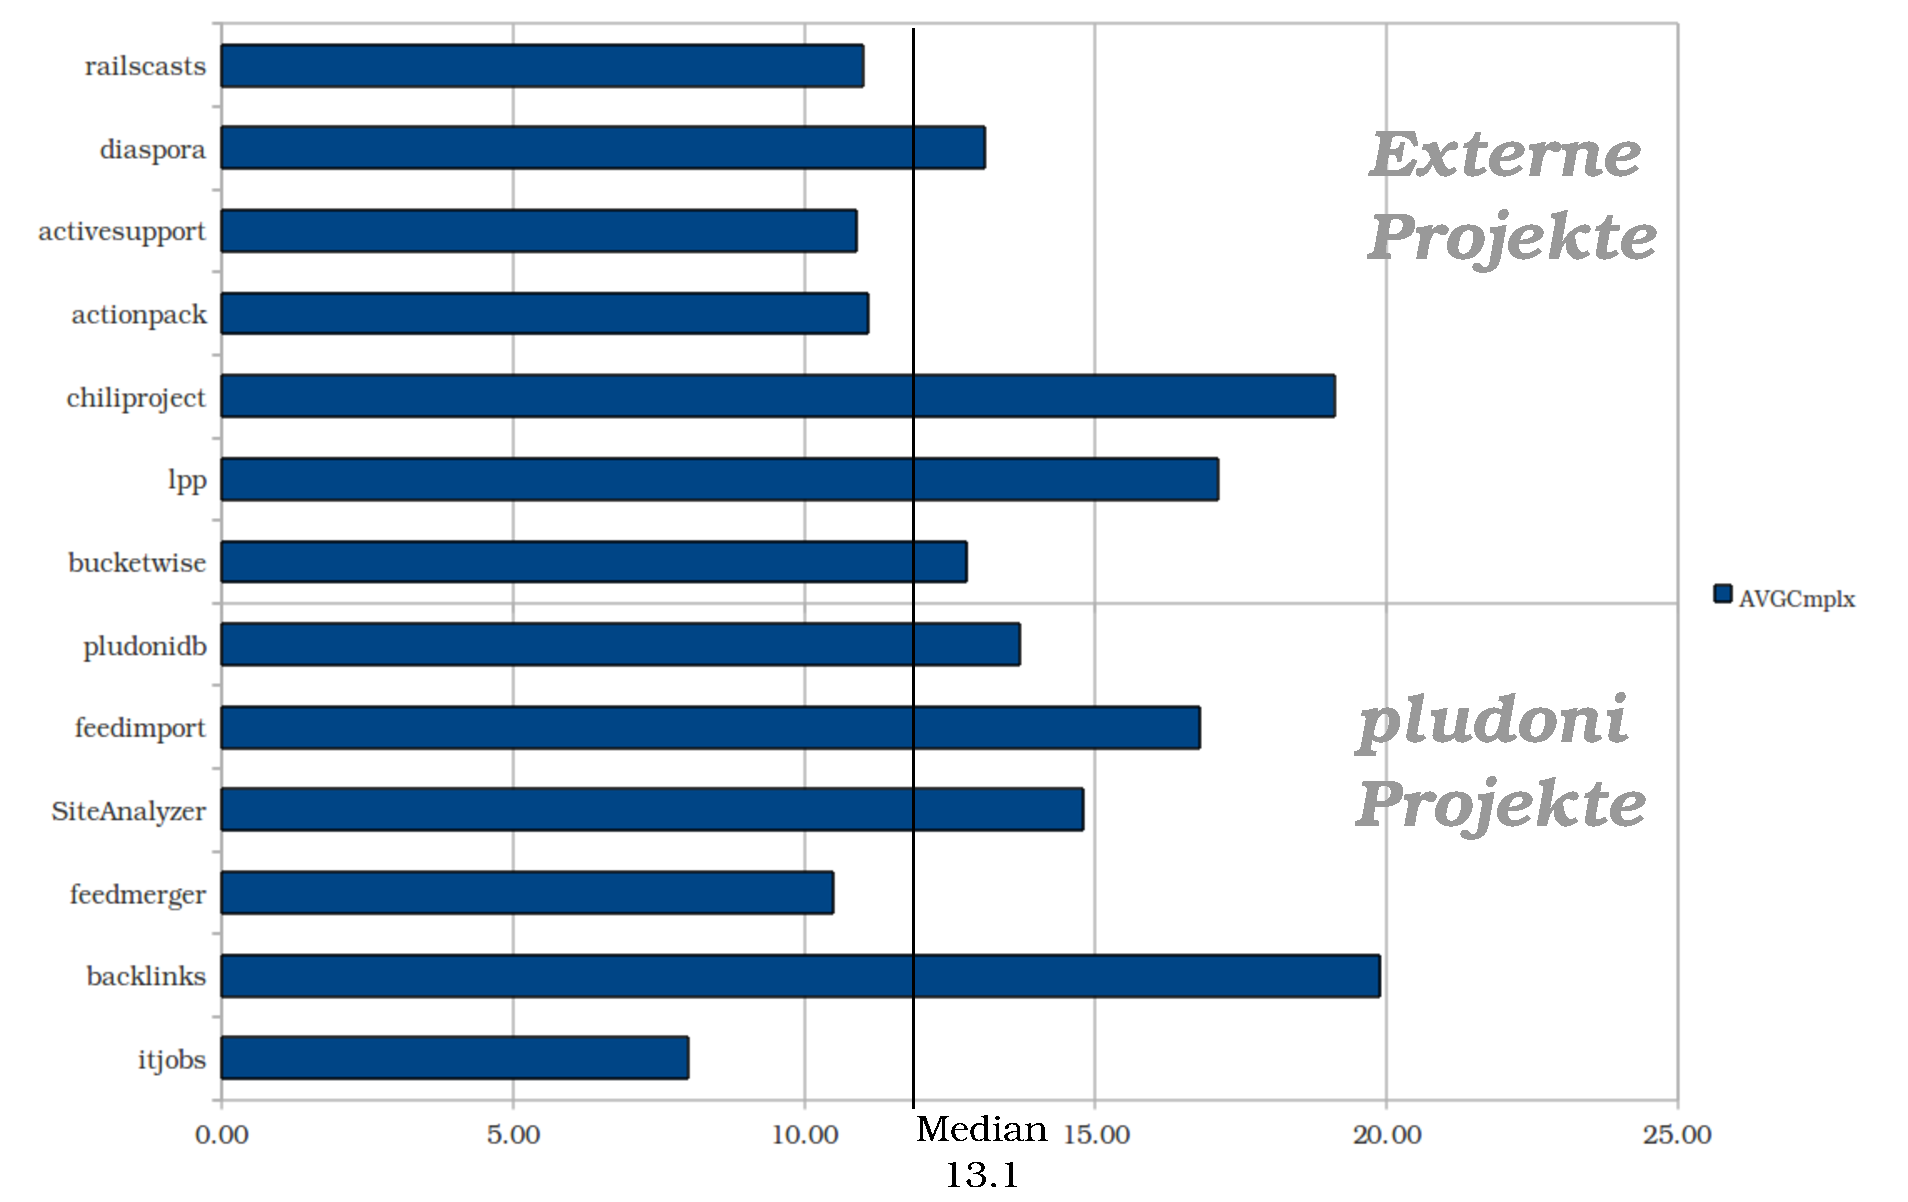
\includegraphics[width=\linewidth]{./diagrams/cmp-complex.pdf}
 % cpm-lotloc.pdf: 930x574 pixel, 72dpi, 32.81x20.25 cm, bb=0 0 930 574
 \caption{Vergleich der durchschnittlichen Komplexität}
 \label{fig:cpm-complex}
\end{figure}

\begin{figure}[htbp]
 \centering
 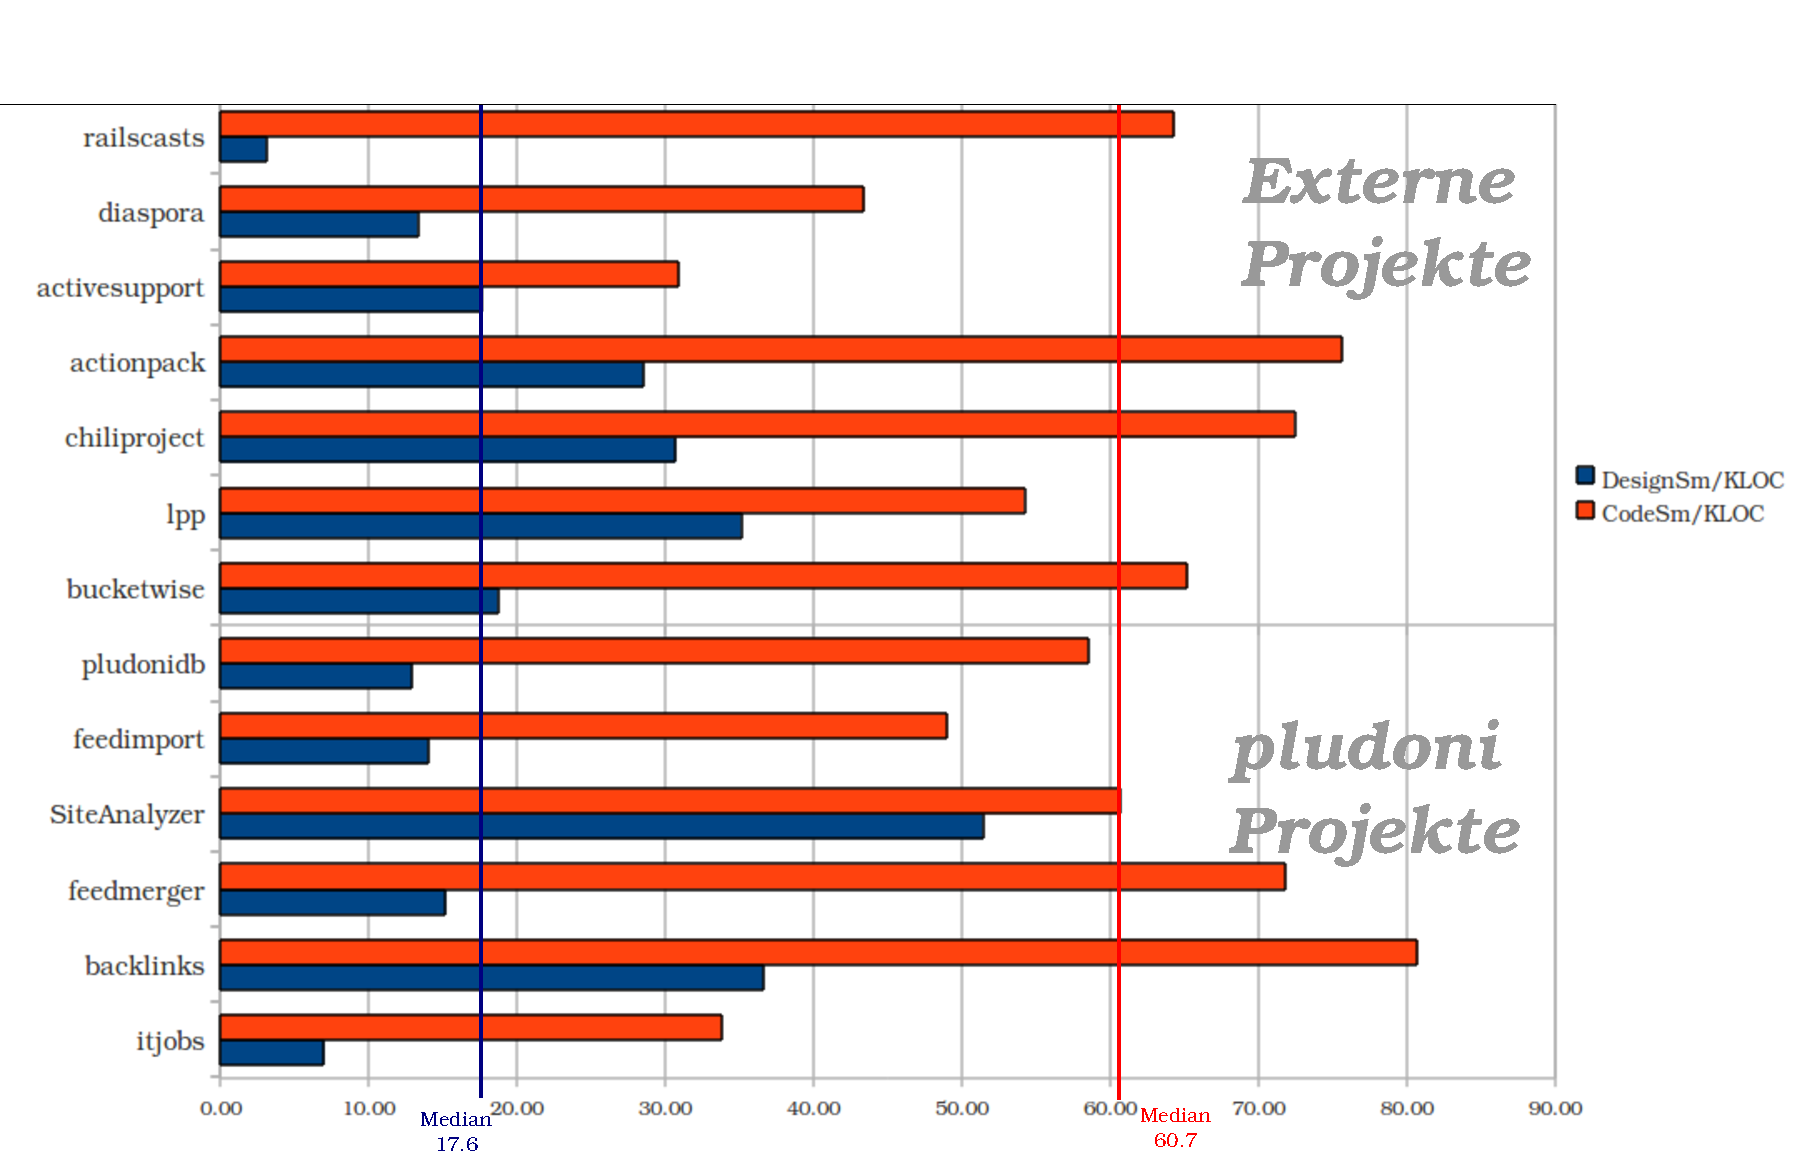
\includegraphics[width=\linewidth]{./diagrams/cpm-smells.pdf}
 % cpm-lotloc.pdf: 930x574 pixel, 72dpi, 32.81x20.25 cm, bb=0 0 930 574
 \caption{Vergleich der Anzahl Smells pro KLOC}
 \label{fig:cpm-complex}
\end{figure}





